\documentclass[11pt]{article}
\usepackage[margin=1in]{geometry}
\usepackage{booktabs, tabularx}
\usepackage{pgfplots}
\pgfplotsset{compat=1.18}
\usepackage{tikz}
\usetikzlibrary{positioning, arrows.meta, shapes.geometric, decorations.pathreplacing}
\usepackage{hyperref}
\usepackage{amsmath}
\usepackage[table]{xcolor}
\usepackage{enumitem}
\usepackage[T1]{fontenc}
\usepackage{microtype}
\usepackage{parskip}

% Colors
\definecolor{dblue}{HTML}{003366}
\definecolor{dgreen}{HTML}{2D8F2D}
\definecolor{dred}{HTML}{CC3333}
\definecolor{dorange}{HTML}{E68A00}
\definecolor{dgray}{HTML}{666666}
\definecolor{lblue}{HTML}{4A90D9}
\definecolor{lgreen}{HTML}{66BB6A}
\definecolor{lred}{HTML}{EF5350}
\definecolor{lpurple}{HTML}{AB47BC}
\definecolor{cblue}{HTML}{1976D2}
\definecolor{cred}{HTML}{E64A19}
\definecolor{cgray}{HTML}{757575}

\hypersetup{colorlinks=true, linkcolor=dblue, urlcolor=dblue}

\title{\textbf{Progress Update: Cross-Patient Speech Decoding}}
\author{Ben Tang \\ Cogan Lab, Duke}
\date{April 6, 2026}

\begin{document}
\maketitle
\thispagestyle{empty}

\noindent\textit{Summary:} A neural network pipeline was built for per-patient phoneme decoding, achieving PER 0.734 on S14 with grouped cross-validation. Self-supervised learning (SSL) was tested to pool data across patients --- it failed because only $\sim$11 minutes of epoched data are available. However, \textbf{456 minutes of raw continuous recordings} exist across 29 patients. Combined with a new architecture that uses \textbf{brain coordinates} to align electrodes across patients, this opens a path to cross-patient decoding.

\bigskip
\hrule
\bigskip

%% ============================================================
\section{Starting Point}
%% ============================================================

Quick recap of the setup:

\begin{itemize}[nosep]
    \item \textbf{Task:} Non-word repetition --- 52 CVC/VCV tokens, 3 phonemes each, 9 phoneme classes
    \item \textbf{Data:} 11 patients, 46--178 trials each, $\sim$1 minute of speech per patient
    \item \textbf{Prior baseline (Spalding 2025):} PCA $\to$ CCA $\to$ SVM --- cross-patient balanced accuracy \textbf{0.31} (chance = 0.11)
    \item \textbf{Metric:} Phoneme Error Rate (PER). Lower is better. Chance = 0.889 for 9-way.
\end{itemize}

All results use \textbf{grouped-by-token cross-validation} --- all 3 phoneme positions of a token stay in the same fold. Stratified CV leaks information across folds and inflates results by $\sim$10 percentage points.

%% ============================================================
\section{Neural Network Pipeline}
%% ============================================================

The new pipeline, built in PyTorch, uses the 2D spatial layout of the electrode grid instead of flattening channels.

\begin{figure}[ht]
\centering
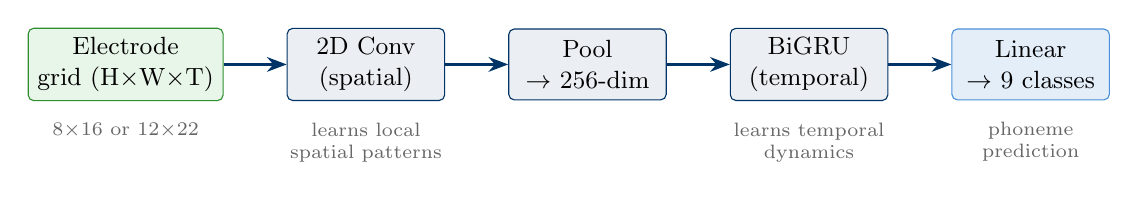
\begin{tikzpicture}[
    block/.style={rectangle, draw=dblue, fill=dblue!8, minimum height=0.9cm, minimum width=2cm, align=center, font=\small, rounded corners=2pt},
    arr/.style={-{Stealth[length=2.5mm]}, thick, dblue},
]
\node[block, fill=lgreen!15, draw=dgreen] (input) {Electrode\\grid (H$\times$W$\times$T)};
\node[block, right=0.8cm of input] (conv) {2D Conv\\(spatial)};
\node[block, right=0.8cm of conv] (pool) {Pool\\$\to$ 256-dim};
\node[block, right=0.8cm of pool] (gru) {BiGRU\\(temporal)};
\node[block, right=0.8cm of gru, fill=lblue!15, draw=lblue] (head) {Linear\\$\to$ 9 classes};

\draw[arr] (input) -- (conv);
\draw[arr] (conv) -- (pool);
\draw[arr] (pool) -- (gru);
\draw[arr] (gru) -- (head);

\node[font=\scriptsize, text=dgray, below=0.15cm of input] {8$\times$16 or 12$\times$22};
\node[font=\scriptsize, text=dgray, align=center, below=0.15cm of conv] {learns local\\spatial patterns};
\node[font=\scriptsize, text=dgray, align=center, below=0.15cm of gru] {learns temporal\\dynamics};
\node[font=\scriptsize, text=dgray, align=center, below=0.15cm of head] {phoneme\\prediction};
\end{tikzpicture}
\caption{Per-patient pipeline. Each patient gets their own spatial Conv2d (because their grid is physically different), but the temporal backbone (BiGRU) and classifier head are shared.}
\label{fig:pipeline}
\end{figure}

\subsection{Key Changes That Helped}

Starting from the basic pipeline, several changes were tuned on patient S14:

\begin{enumerate}[nosep]
    \item \textbf{Switched CTC $\to$ cross-entropy loss} (+7.8pp). CTC tries to learn alignment \textit{and} classification simultaneously --- with only $\sim$150 trials, that's too much to ask.
    \item \textbf{Increased spatial pooling} (pool 2$\times$4 $\to$ 4$\times$8). The original preserved 4mm spatial resolution, but phoneme-relevant somatotopy is at 3--5mm scale --- we were keeping noise.
    \item \textbf{Per-phoneme MFA epochs.} Instead of one epoch per trial (with all 3 phonemes), each trial is cut into 3 separate epochs aligned to each phoneme's onset using the MFA timestamps. This triples the labeled samples and gives a single-phoneme classification target. Won on \textbf{8 of 11 patients}.
    \item \textbf{Evaluation recipe:} focal loss, label smoothing, mixup augmentation, weighted k-NN on learned features, test-time augmentation. Each added 1--3pp.
\end{enumerate}

\begin{figure}[ht]
\centering
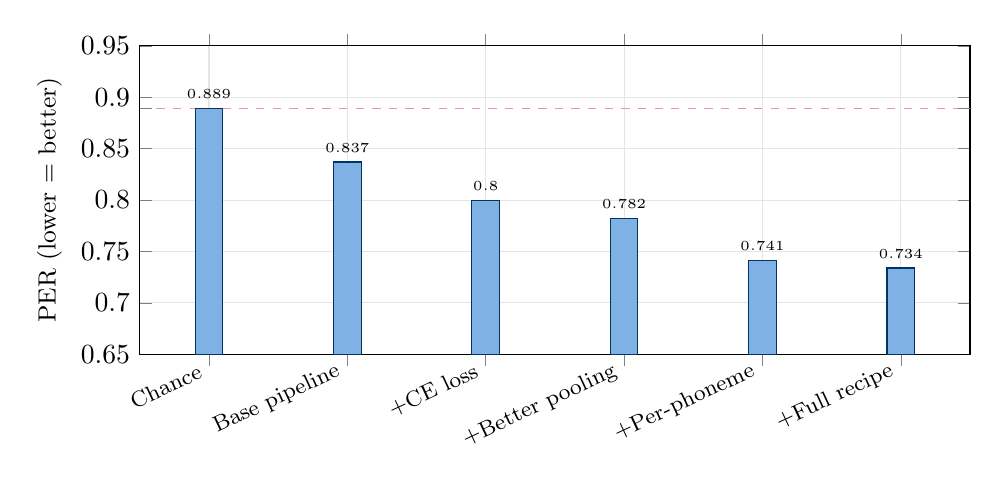
\begin{tikzpicture}
\begin{axis}[
    width=\textwidth,
    height=5.5cm,
    ybar,
    bar width=10pt,
    ylabel={PER (lower = better)},
    ylabel style={font=\small},
    symbolic x coords={Chance,{Base pipeline},{+CE loss},{+Better pooling},{+Per-phoneme},{+Full recipe}},
    xtick=data,
    x tick label style={rotate=25, anchor=east, font=\footnotesize},
    ymin=0.65, ymax=0.95,
    ytick={0.65,0.70,...,0.95},
    nodes near coords,
    nodes near coords style={font=\tiny, above},
    every node near coord/.append style={/pgf/number format/.cd, fixed, precision=3},
    grid=major,
    grid style={gray!20},
    extra y ticks={0.889},
    extra y tick labels={},
    extra y tick style={grid=major, grid style={dashed, dred!50}},
]
\addplot[fill=lblue!70, draw=dblue] coordinates {
    (Chance, 0.889)
    ({Base pipeline}, 0.837)
    ({+CE loss}, 0.800)
    ({+Better pooling}, 0.782)
    ({+Per-phoneme}, 0.741)
    ({+Full recipe}, 0.734)
};
\end{axis}
\end{tikzpicture}
\caption{\textbf{Per-patient results on S14} (grouped CV, best configuration at each step). Each bar shows the cumulative effect of adding one improvement. The biggest single gain was switching to per-phoneme MFA epochs.}
\label{fig:progression}
\end{figure}

\subsection{Per-Phoneme Results Across All 11 Patients}

Per-phoneme MFA generalizes beyond S14 --- it helps most patients:

\begin{figure}[ht]
\centering
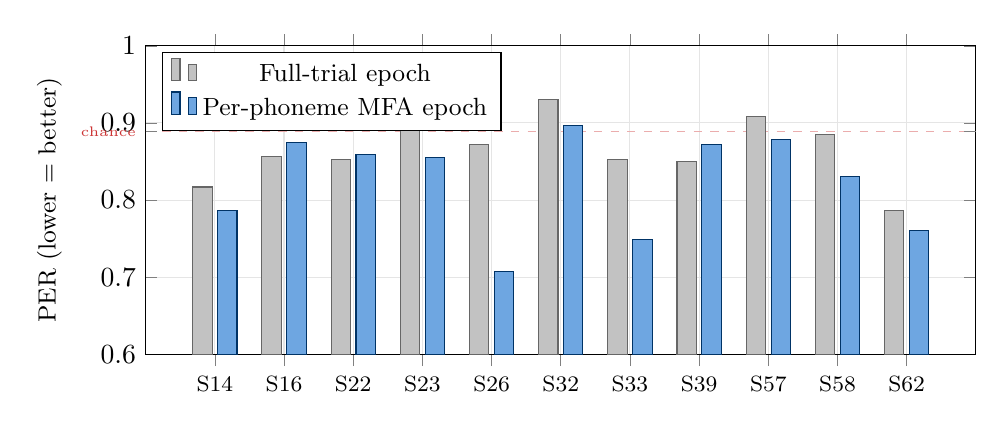
\begin{tikzpicture}
\begin{axis}[
    width=\textwidth,
    height=5.5cm,
    ybar,
    bar width=7pt,
    ylabel={PER (lower = better)},
    ylabel style={font=\small},
    symbolic x coords={S14,S16,S22,S23,S26,S32,S33,S39,S57,S58,S62},
    xtick=data,
    x tick label style={font=\footnotesize},
    ymin=0.60, ymax=1.0,
    legend style={at={(0.02,0.98)}, anchor=north west, font=\small},
    grid=major,
    grid style={gray!20},
    extra y ticks={0.889},
    extra y tick labels={chance},
    extra y tick style={grid=major, grid style={dashed, dred!40}, tick label style={font=\tiny, text=dred}},
]
\addplot[fill=dgray!40, draw=dgray] coordinates {
    (S14, 0.817) (S16, 0.857) (S22, 0.853) (S23, 0.905) (S26, 0.872)
    (S32, 0.930) (S33, 0.853) (S39, 0.850) (S57, 0.908) (S58, 0.885) (S62, 0.786)
};
\addplot[fill=lblue!80, draw=dblue] coordinates {
    (S14, 0.786) (S16, 0.875) (S22, 0.859) (S23, 0.855) (S26, 0.707)
    (S32, 0.897) (S33, 0.749) (S39, 0.872) (S57, 0.879) (S58, 0.831) (S62, 0.761)
};
\legend{Full-trial epoch, Per-phoneme MFA epoch}
\end{axis}
\end{tikzpicture}
\caption{\textbf{Per-phoneme wins 8/11 patients.} Population mean: 0.825 vs 0.865 (+4pp). Biggest gains on S26 (+16.5pp) and S33 (+10.4pp). The 3 patients where full-trial wins (S16, S22, S39) have poor MFA alignment --- the phoneme onsets are off by 300--500ms.}
\label{fig:multipatient}
\end{figure}

\textbf{Best per-patient result (S14, 3-seed):} PER \textbf{0.734 $\pm$ 0.007}.

\textbf{Caveat:} Per-phoneme epochs have 85\% temporal overlap (consecutive phoneme onsets are only $\sim$80ms apart in a 650ms window). The ``3$\times$ more samples'' is more like 1.3$\times$ independent data. Trial-aware batching (never placing epochs from the same trial in the same batch) mitigates this.

%% ============================================================
\section{Cross-Patient: Why It's Hard}
%% ============================================================

Per-patient decoding is useful, but the real goal is cross-patient transfer. \textbf{55 experiments} were run testing different cross-patient approaches (leave-one-patient-out: train on 10, test on 1).

\textbf{Result:} Everything converged to PER $\sim$0.750, regardless of approach.

\begin{figure}[ht]
\centering
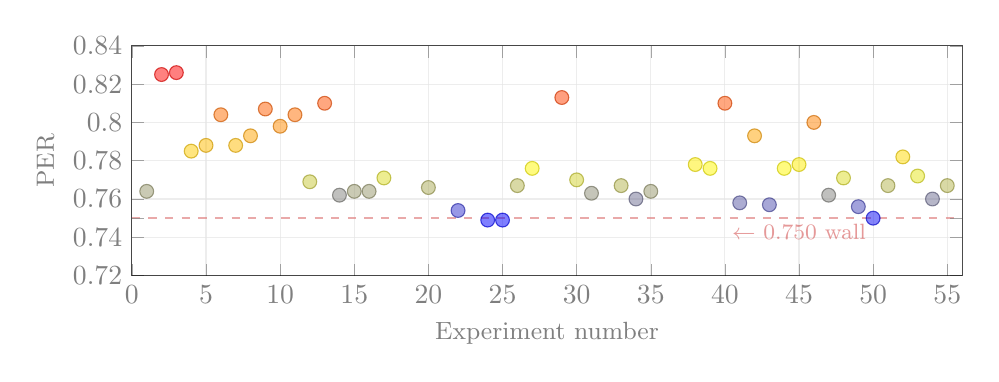
\begin{tikzpicture}
\begin{axis}[
    width=\textwidth,
    height=4.5cm,
    scatter,
    only marks,
    xlabel={Experiment number},
    ylabel={PER},
    ylabel style={font=\small},
    xlabel style={font=\small},
    xmin=0, xmax=56,
    ymin=0.72, ymax=0.84,
    ytick={0.72,0.74,...,0.84},
    grid=major,
    grid style={gray!20},
    extra y ticks={0.750},
    extra y tick labels={},
    extra y tick style={grid=major, grid style={thick, dashed, dred!60}},
    mark=*,
    mark size=2.5pt,
    draw opacity=0.7,
    fill opacity=0.5,
]
\addplot[lblue, mark=*, fill=lblue!60] coordinates {
    (1,0.764) (2,0.825) (3,0.826) (4,0.785) (5,0.788) (6,0.804) (7,0.788)
    (8,0.793) (9,0.807) (10,0.798) (11,0.804) (12,0.769) (13,0.810)
    (14,0.762) (15,0.764) (16,0.764) (17,0.771)
    (20,0.766) (22,0.754) (24,0.749) (25,0.749) (26,0.767) (27,0.776)
    (29,0.813) (30,0.770) (31,0.763) (33,0.767) (34,0.760) (35,0.764)
    (38,0.778) (39,0.776) (40,0.810) (41,0.758) (42,0.793) (43,0.757)
    (44,0.776) (45,0.778) (46,0.800) (47,0.762) (48,0.771)
    (49,0.756) (50,0.750) (51,0.767) (52,0.782) (53,0.772) (54,0.760) (55,0.767)
};
\node[font=\footnotesize, text=dred] at (axis cs:45,0.743) {$\leftarrow$ 0.750 wall};
\end{axis}
\end{tikzpicture}
\caption{\textbf{55 cross-patient experiments all land in the same range.} Variations tested: learning rates, architectures (transformers, LSTMs), domain adaptation (CORAL, gradient reversal), backbone sizes, multi-scale temporal convolutions. Nothing broke through the $\sim$0.750 wall.}
\label{fig:lopo}
\end{figure}

\subsection{The Real Problem: Electrodes Don't Overlap}

Why is cross-patient so hard? Computing the actual distances between every pair of patients' electrode arrays in MNI brain coordinates reveals the answer.

\textbf{Mean distance between array centers: 36mm.} Most patient pairs have essentially zero electrode overlap.

\begin{figure}[ht]
\centering
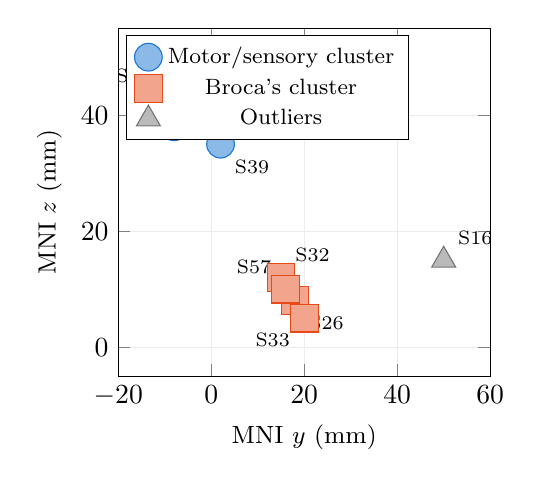
\begin{tikzpicture}
\begin{axis}[
    width=0.52\textwidth,
    height=6cm,
    xlabel={MNI $y$ (mm)},
    ylabel={MNI $z$ (mm)},
    xlabel style={font=\small},
    ylabel style={font=\small},
    xmin=-20, xmax=60,
    ymin=-5, ymax=55,
    grid=major,
    grid style={gray!15},
    legend style={at={(0.02,0.98)}, anchor=north west, font=\footnotesize},
]
% Posterior-dorsal cluster (motor/sensory cortex)
\addplot[only marks, mark=*, mark size=5pt, draw=cblue, fill=cblue!50] coordinates {
    (-5,42) (-8,38) (2,35) (-3,40) (-10,43)
};
% Anterior-ventral cluster (Broca's area)
\addplot[only marks, mark=square*, mark size=5pt, draw=cred, fill=cred!50] coordinates {
    (18,8) (15,12) (20,5) (16,10)
};
% Outliers
\addplot[only marks, mark=triangle*, mark size=5pt, draw=cgray, fill=cgray!50] coordinates {
    (50,15) (-2,40)
};
% Labels
\node[font=\scriptsize, anchor=south west] at (axis cs:-4,43) {S14};
\node[font=\scriptsize, anchor=south east] at (axis cs:-9,39) {S23};
\node[font=\scriptsize, anchor=north west] at (axis cs:3,34) {S39};
\node[font=\scriptsize, anchor=south] at (axis cs:-3,41) {S58};
\node[font=\scriptsize, anchor=south east] at (axis cs:-11,44) {S62};
\node[font=\scriptsize, anchor=north west] at (axis cs:19,7) {S26};
\node[font=\scriptsize, anchor=south west] at (axis cs:16,13) {S32};
\node[font=\scriptsize, anchor=north east] at (axis cs:19,4) {S33};
\node[font=\scriptsize, anchor=south east] at (axis cs:15,11) {S57};
\node[font=\scriptsize, anchor=south west] at (axis cs:51,16) {S16};
\node[font=\scriptsize, anchor=south west] at (axis cs:-1,41) {S22};
\legend{Motor/sensory cluster, Broca's cluster, Outliers}
\end{axis}
\end{tikzpicture}
\hfill
\begin{minipage}[b]{0.42\textwidth}
\centering
\small
\begin{tabular}{lr}
\toprule
& Distance \\
\midrule
Mean between arrays & \textbf{36 mm} \\
Range & 8.5--75.6 mm \\
Pairs with overlap & 9/55 \\
\midrule
\multicolumn{2}{l}{\textit{Closest pairs:}} \\
S26 $\leftrightarrow$ S33 & 1.3 mm \\
S22 $\leftrightarrow$ S62 & 2.7 mm \\
\midrule
\multicolumn{2}{l}{\textit{Farthest pairs:}} \\
S16 $\leftrightarrow$ S14 & 75.6 mm \\
\bottomrule
\end{tabular}

\vspace{0.5em}
\footnotesize
The two clusters cover \textit{different brain regions}: one is on motor/sensory cortex, the other on Broca's area. These regions encode speech in fundamentally different ways --- so a model trained on one cluster has limited transfer to the other.
\end{minipage}
\caption{\textbf{Where each patient's electrode array sits on the brain} (MNI coordinates, lateral view). Arrays are placed by the surgeon for clinical reasons, not experimentally standardized. The current pipeline (Conv2d) treats each grid as an abstract image --- it has no idea where on the brain the electrodes actually are.}
\label{fig:overlap}
\end{figure}

\textbf{Key insight:} The current pipeline maps each patient's electrode grid to a shared feature space using 2D convolution. But it treats the grid as an abstract image with no knowledge of brain location. When patient A's electrodes sit on motor cortex and patient B's sit on Broca's area, the shared backbone has no way to account for this --- it's comparing apples to oranges.

%% ============================================================
\section{SSL Attempt: Not Enough Data}
%% ============================================================

Self-supervised pretraining (SSL) was also tested --- the idea being that learning general neural signal structure from unlabeled data might improve cross-patient transfer.

Six methods were evaluated (JEPA, BYOL, DINO, VICReg, LeWM, and masked reconstruction):

\begin{figure}[ht]
\centering
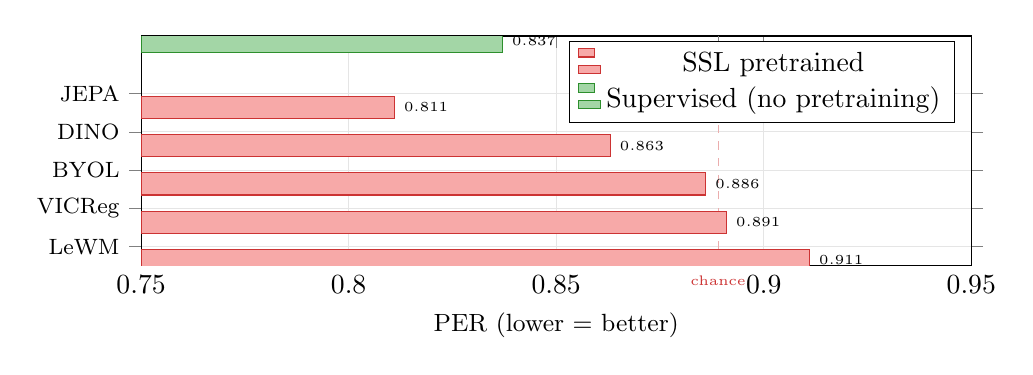
\begin{tikzpicture}
\begin{axis}[
    width=\textwidth,
    height=4.5cm,
    xbar,
    bar width=8pt,
    xlabel={PER (lower = better)},
    xlabel style={font=\small},
    symbolic y coords={LeWM,VICReg,BYOL,DINO,JEPA,Supervised},
    ytick=data,
    y tick label style={font=\footnotesize},
    xmin=0.75, xmax=0.95,
    xtick={0.75,0.80,...,0.95},
    grid=major,
    grid style={gray!20},
    extra x ticks={0.889},
    extra x tick labels={chance},
    extra x tick style={grid=major, grid style={dashed, dred!40}, tick label style={font=\tiny, text=dred}},
    nodes near coords,
    nodes near coords style={font=\tiny, anchor=west},
    every node near coord/.append style={/pgf/number format/.cd, fixed, precision=3},
]
\addplot[fill=lred!50, draw=dred] coordinates {
    (0.911,LeWM)
    (0.891,VICReg)
    (0.886,BYOL)
    (0.863,DINO)
    (0.811,JEPA)
};
\addplot[fill=lgreen!60, draw=dgreen] coordinates {
    (0.837,Supervised)
};
\legend{SSL pretrained, Supervised (no pretraining)}
\end{axis}
\end{tikzpicture}
\caption{\textbf{Every SSL method performed worse than simply training with labels.} Best SSL: JEPA with k-NN evaluation (0.811). The green bar is the supervised baseline (0.837) --- no pretraining at all. SSL needs a minimum of $\sim$30 minutes of data to help (based on prior ECoG work), and we only have $\sim$11 minutes of epoched data.}
\label{fig:ssl}
\end{figure}

\textbf{Why SSL failed:} The dataset contains only $\sim$11 minutes of epoched neural data across 11 patients. Prior work (wav2vec on ECoG) found that SSL needs at least $\sim$30 minutes to provide benefit --- 3$\times$ more than what was available.

\textbf{However:}

%% ============================================================
\section{The Unlock: 456 Minutes of Raw Continuous Data}
%% ============================================================

The raw continuous EDF recordings on the BIDS server contain far more data than just the epoched trials:

\begin{table}[ht]
\centering
\begin{tabular}{lrrl}
\toprule
Dataset & Patients & Duration & Notes \\
\midrule
PS (our task) & 13 & 199 min & Same task, more patients than the 11 we epoch \\
Lexical (word/nonword) & 17 & 257 min & Different task, zero patient overlap with PS \\
\midrule
\textbf{Total} & \textbf{29} & \textbf{456 min} & \textbf{15$\times$ the SSL threshold} \\
\bottomrule
\end{tabular}
\caption{Raw continuous recordings available. The 17 Lexical patients provide completely independent neural data for self-supervised pretraining --- same electrode hardware, same cortical regions, different task.}
\label{tab:continuous}
\end{table}

This changes the SSL picture entirely. With 456 minutes (7.6 hours), the dataset is well above the threshold where SSL starts helping. The 17 Lexical patients provide independent neural recordings from the same type of electrode arrays on the same brain regions.

\textbf{The catch:} These are raw 2kHz voltage recordings. High-gamma activity (HGA) features need to be extracted to match the existing pipeline. This requires running IEEG\_Pipelines preprocessing (CAR $\to$ 70--150Hz filterbank $\to$ Hilbert envelope $\to$ downsample to 200Hz).

%% ============================================================
\section{Hypothesis: Brain Coordinates Can Break the Wall}
%% ============================================================

The 55-experiment wall and the electrode overlap analysis suggest the same bottleneck: \textbf{the current pipeline has no knowledge of where electrodes sit in the brain.} The Conv2d treats each patient's grid as an abstract image. When one patient's array covers motor cortex and another's covers Broca's area, the shared backbone has no mechanism to account for this.

The hypothesis: \textbf{if each electrode is tagged with its MNI brain coordinates, cross-patient transfer should improve}, because the model can learn that ``activity at face motor cortex'' means the same thing regardless of which patient it comes from.

But this hypothesis needs to be tested incrementally. There are several ways to incorporate coordinates, ranging from trivial to complex. Jumping to the most complex architecture without validating simpler alternatives would not be rigorous.

\subsection{Ablation Ladder}

Each step adds exactly one thing. If an early step fails, everything after it is unlikely to help.

\begin{center}
\small
\begin{tabularx}{\textwidth}{c>{\raggedright\arraybackslash}p{5cm}>{\raggedright\arraybackslash}X}
\toprule
Step & What changes & What it tests \\
\midrule
A0 & Current Conv2d pipeline (LOPO) & Baseline: PER $\sim$0.750 \\[0.3em]
A1 & Add patient's array MNI centroid as global conditioning & Does even \textit{coarse} spatial info help? (3 numbers per patient, minimal code change) \\[0.3em]
A2 & Flatten grid $\to$ per-electrode tokens with raw MNI $(x,y,z)$ & Do fine-grained coordinates carry signal? Requires abandoning 2D conv for a set model. \\[0.3em]
A3 & Replace raw $(x,y,z)$ with Fourier positional encoding & Does multi-scale encoding help? Wavelengths 30, 15, 7.5mm --- shortest near MNI noise floor. \\[0.3em]
A4 & Cross-attention to 10 fixed Brainnetome atlas positions & Does anatomical aggregation add value beyond raw coordinates? Or equivalent to spatial pooling? \\[0.3em]
A5 & Initialize VEs at atlas, allow gradient descent to move them & Is the atlas correct? If positions drift $>$10mm, atlas centroids were a bad prior. \\[0.3em]
A6 & Add reconstruction loss at masked electrodes & Does spatial self-supervision help? Can train on all 456 min continuous data. \\
\bottomrule
\end{tabularx}
\end{center}

\textbf{Key decision points:}
\begin{itemize}[nosep]
    \item If A1 already helps $\to$ even coarse spatial info is useful; proceed down the ladder.
    \item If A2 doesn't beat A0 $\to$ MNI coordinates are too noisy at uECOG scale; stop and reconsider.
    \item If A4 $\approx$ A3 $\to$ the virtual electrode aggregation adds no value over raw coordinates; use the simpler model.
    \item If A5 positions drift far from atlas $\to$ fixed atlas positions are a bad assumption; use learned positions.
\end{itemize}

\subsection{The Target Architecture (If Ablations Support It)}

If the ablation ladder validates that coordinates and spatial aggregation both help, the full architecture looks like this:

\begin{figure}[ht]
\centering
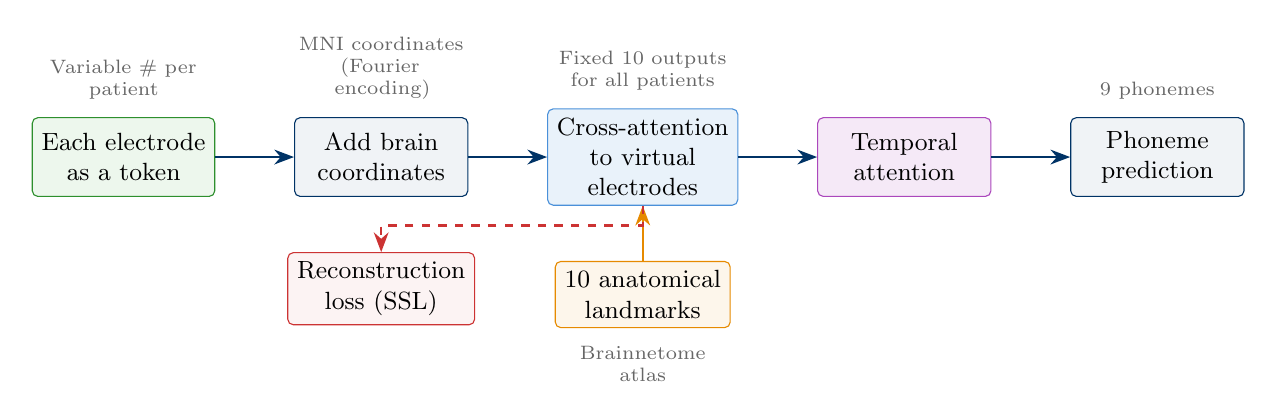
\begin{tikzpicture}[
    block/.style={rectangle, draw=dblue, fill=dblue!6, minimum height=1cm, minimum width=2.2cm, align=center, font=\small, rounded corners=2pt},
    arr/.style={-{Stealth[length=2.5mm]}, thick, dblue},
    note/.style={font=\scriptsize, text=dgray, align=center, text width=2.2cm},
]

% Blocks
\node[block, fill=lgreen!12, draw=dgreen] (input) {Each electrode\\as a token};
\node[block, right=1cm of input] (fpe) {Add brain\\coordinates};
\node[block, right=1cm of fpe, fill=lblue!12, draw=lblue] (xattn) {Cross-attention\\to virtual\\electrodes};
\node[block, right=1cm of xattn, fill=lpurple!12, draw=lpurple] (tattn) {Temporal\\attention};
\node[block, right=1cm of tattn] (out) {Phoneme\\prediction};

% Virtual electrodes box
\node[rectangle, draw=dorange, fill=dorange!8, minimum height=0.7cm, minimum width=1.8cm, align=center, font=\small, rounded corners=2pt, below=0.7cm of xattn] (ve) {10 anatomical\\landmarks};
\node[note, below=0.1cm of ve] {Brainnetome atlas};

% Reconstruction loss
\node[rectangle, draw=dred, fill=dred!6, minimum height=0.7cm, minimum width=1.6cm, align=center, font=\small, rounded corners=2pt, below=0.7cm of fpe] (recon) {Reconstruction\\loss (SSL)};

% Arrows
\draw[arr] (input) -- (fpe);
\draw[arr] (fpe) -- (xattn);
\draw[arr] (xattn) -- (tattn);
\draw[arr] (tattn) -- (out);
\draw[arr, dorange] (ve) -- (xattn);
\draw[arr, dashed, dred] (xattn.south) -- ++(0,-0.25) -| (recon.north);

% Notes
\node[note, above=0.1cm of input] {Variable \# per\\patient};
\node[note, above=0.1cm of fpe] {MNI coordinates\\(Fourier encoding)};
\node[note, above=0.1cm of xattn] {Fixed 10 outputs\\for all patients};
\node[note, above=0.1cm of out] {9 phonemes};

\end{tikzpicture}
\caption{\textbf{Target architecture (contingent on ablation results).} Each electrode becomes a token tagged with its MNI brain coordinates. Cross-attention maps these to a fixed set of virtual electrodes at anatomical positions. The reconstruction loss enables self-supervised pretraining on the 456 min of continuous data. This is \textbf{step A4--A6} of the ablation ladder --- only pursued if steps A1--A3 validate that coordinates help.}
\label{fig:v12}
\end{figure}

\subsection{Known Risks}

Several assumptions in the full architecture have not been validated:

\begin{itemize}[nosep]
    \item \textbf{MNI coordinate accuracy.} Registration error is 5--10mm, but electrode spacing is only 1.3--1.7mm. Coordinates may be too noisy to distinguish neighboring electrodes at uECOG scale. Chen 2025 validated coordinates at 1cm ECoG spacing --- a different regime. Ablation step A2 directly tests this.
    \item \textbf{Atlas centroids as fixed positions.} Brainnetome centroids are population averages. Individual functional boundaries vary by 5--15mm, and some patients have tumors that distort anatomy. Step A5 tests whether learned positions outperform atlas positions.
    \item \textbf{Cross-attention vs simpler pooling.} With $\sim$100 electrodes and 4--6 active VEs per patient, each VE is effectively a distance-weighted average of $\sim$20 electrodes. This might not be meaningfully different from learned spatial pooling. Step A4 vs A3 tests this directly.
    \item \textbf{Is the wall even about spatial alignment?} The 0.750 wall could reflect insufficient training data ($\sim$1300 trials from 10 patients), evaluation noise (30 validation samples/fold), or backbone capacity. If the wall breaks with more data alone, the coordinate-based approach is solving the wrong problem. The SSL experiments on continuous data (step A6) help distinguish these explanations.
\end{itemize}

\subsection{What's Not In Question}

The analysis and atlas work done so far is reusable regardless of which architecture step wins:

\begin{itemize}[nosep]
    \item \textbf{Brainnetome atlas.} Only atlas separating tongue vs lip vs laryngeal motor cortex. Even if fixed VEs don't work, the ROI definitions inform analysis and interpretability.
    \item \textbf{Coverage analysis.} 6/16 ROIs unreachable, 10 reachable, patient-adaptive selection --- this applies to any coordinate-based approach.
    \item \textbf{Coordinate pipeline.} ACPC $\to$ MNI transforms, chanMap integration, hemisphere mirroring --- needed for any model that uses brain location.
    \item \textbf{456 min continuous data.} Useful for SSL regardless of architecture choice.
\end{itemize}

%% ============================================================
\section{Data Quality Issues Found}
%% ============================================================

A systematic data audit also revealed:

\begin{itemize}[nosep]
    \item \textbf{Artifact channels:} S39 (20 channels), S57 (15), S58 (37) have electronic artifacts from mic feedback / amplifier saturation --- confirmed not brain signal. These need to be excluded (currently just zeroed in the grid).
    \item \textbf{MFA quality:} 3 patients (S16, S22, S39) have poor phoneme onset alignment (300--500ms off). Plan: start with the 8 good patients, add these later with full-trial epochs as fallback.
    \item \textbf{Coordinate mapping:} 128-channel patients require the chanMap file to correctly map amplifier channels to physical electrode positions. Without it, there's an 8.5mm error. This is now implemented and verified.
    \item \textbf{S32/S57 sigChannel:} Missing significance channel masks for these two patients. Not blocking --- all non-artifact channels can be used instead.
\end{itemize}

%% ============================================================
\section{Open Questions \& Blockers}
%% ============================================================

\begin{enumerate}
    \item \textbf{Continuous HGA extraction (main blocker).} The 456 minutes of raw EDFs need HGA extraction via \texttt{extractHiGamma()} or the Python equivalent (\texttt{ieeg.timefreq.gamma.extract()}). This is the single biggest unlock --- both for SSL and for testing whether more data alone breaks the 0.750 wall.

    \item \textbf{S32/S57 sigChannel.} Are these significance channel masks recoverable? Not urgent --- the pipeline can proceed without them.

    \item \textbf{Coordinate-based direction.} Does using brain coordinates for cross-patient alignment make sense given the data? The ablation ladder (A0--A6) is designed to validate this incrementally rather than committing to the full architecture upfront.

    \item \textbf{MFA re-alignment.} For S16/S22/S39 with poor MFA, should MFA be re-run with different parameters, or should those patients fall back to full-trial epochs?
\end{enumerate}

\subsection{Timeline}

\begin{enumerate}[nosep]
    \item \textbf{This week:} Begin continuous HGA extraction if unblocked. Implement ablation step A1 (centroid conditioning --- minimal code change).
    \item \textbf{Next 2 weeks:} Run A1--A3 on Duke cluster. These are fast experiments that validate or kill the coordinate hypothesis before committing to the full architecture.
    \item \textbf{This month:} If coordinates help, build A4--A6. Compare against per-patient baseline (PER 0.734) and LOPO baseline (PER 0.750).
\end{enumerate}

\end{document}
